\documentclass[12pt, a4paper]{report}
\usepackage{graphicx, array, amsthm, amssymb, amsmath, algorithm, algpseudocode, float, xcolor, thmtools, thmbox, exercise}
\usepackage[english]{babel}






\makeatletter
\renewcommand\thmbox@headstyle[2]{\bfseries #1}
\makeatother
\newtheorem[style=M,bodystyle=\normalfont]{theorem}{Theorem}
\newtheorem[style=M,bodystyle=\normalfont]{corollary}{Corollary}
\newtheorem[style=M,bodystyle=\normalfont]{lemma}{Lemma}
\newtheorem[style=M,bodystyle=\normalfont]{definition}{Definition}


\title{Software Engineering II\\ \textit{Exercises}}
\author{Christian Rossi}
\date{Academic Year 2023-2024}

\begin{document}

\maketitle

\newpage

\begin{abstract}
    The objective of the course is to teach the principals methods and processes of software engineering needed to develop complex and qualitative software.
     
    The course covers the following arguments:
    \begin{itemize}
        \item Software process and its organization.
        \item Modelling languages.
        \item Requirements analysis and definition.
        \item Software development methods and tools.
        \item Approaches for verify and validate the software.
    \end{itemize}
\end{abstract}

\newpage

\tableofcontents

\newpage

\chapter{Alloy examples}
    \section{Address book}
    Imagine that we are asked to model a very simple address book. The books that contain a bunch of addresses linked to the corresponding names. 
    
    In this example we have three entities, which are: $Name$, $Addr$ and $Book$.
    $addr$ is linking $Name$ to $Addr$ within the context of $Book$. To indicate this relation we use the keyword $lone$ that indicates that each $Name$ can correspond at most one 
    $Addr$. We can resume the previous statements as:
    \begin{algorithmic}[H]
        \State \textbf{sig} Name $\{\}$
        \State \textbf{sig} Addr $\{\}$
        \State \textbf{sig} Book $\{$ 
        \State \:\:\:\:\:\: addr: Name -$>$ \textbf{lone} Addr 
        \State $\}$
    \end{algorithmic}
    This specification creates the following relations: 
    \begin{itemize}
        \item Sets are unary relations.
        \item Scalars are singleton sets.
        \item The ternary relation involving the three predicates.
    \end{itemize}
    We can declare a new predicate with the keyword $pred$. 
    \begin{algorithmic}[H]
        \State \textbf{pred} show $\{\}$
        \State \textbf{run} show \textbf{for} 3 \textbf{but exactly} 1 Book
    \end{algorithmic}
    Where the second line indicates that we need to find at most three elements for every $Book$. The predicate $show$ defined previously is empty and return always $true$. Now we 
    can define a predicate with some argument, for example: 
    \newpage
    \begin{algorithmic}[h]
        \State \textbf{pred} show [b:Book]$\{$
        \State \:\:\:\:\:\: $\#$ b.addr $>$ 1
        \State $\}$
        \State \textbf{run} show \textbf{for} 3 \textbf{but exactly} 1 Book
    \end{algorithmic} 
    The predicate (consistent) in the previous example adds a constraint on the number of $Address$ relations in a given $Book$. 
    The predicate (consistent) in the following example adds a constraint on the number of different $Address$ that appears in the $Book$.
    \begin{algorithmic}[H]
        \State \textbf{pred} show [b:Book]$\{$
        \State \:\:\:\:\:\: $\#$ b.addr $>$ 1
        \State \:\:\:\:\:\: $\#$ Name.(b.addr) $>$ 1
        \State $\}$
        \State \textbf{run} show \textbf{for} 3 \textbf{but exactly} 1 Book
    \end{algorithmic}
    The predicate (inconsistent) in the following example contains the keyword $some$ that indicates the existence of an element. In this case we have only one $Book$ so the tool 
    will say that no instances can be found. 
    \begin{algorithmic}[H]
        \State \textbf{pred} add [b:Book]$\{$
        \State \:\:\:\:\:\: $\#$ b.addr $>$ 1
        \State \:\:\:\:\:\: \textbf{some} n:Name $\mid$ $\#$ n.(b.addr) $>$ 1
        \State $\}$
        \State \textbf{run} show \textbf{for} 3 \textbf{but exactly} 1 Book
    \end{algorithmic} 
    All the previous predicates are static because they doesn't change the signature. In Alloy there are also dynamic predicates for dynamic analysis. For example we can define a 
    predicate that adds an $Address$ and $Name$ to a $Book$ in the following way: 
    \begin{algorithmic}[H]
        \State \textbf{pred} add [b,b':Book, n:Name,a:Addr]$\{$
        \State \:\:\:\:\:\:\:\: b'.addr=b.addr + n -$>$ a
        \State $\}$
        \State \textbf{pred} showAdd [b,b':Book, n:Name,a:Addr]$\{$
        \State \:\:\:\:\:\:\:\: add[b,b',n,a]
        \State \:\:\:\:\:\:\:\: $\#$Name.(b'.addr) $>$ 1
        \State $\}$
        \State \textbf{run} showAdd
    \end{algorithmic} 
    We can now define a predicate for the $Book$ deletions.  
    \begin{algorithmic}[H]
        \State \textbf{pred} del [b,b':Book, n:Name]$\{$
        \State \:\:\:\:\:\:\:\: b'.addr=b.addr - n -$>$ Addr
        \State $\}$
    \end{algorithmic} 
    We can check if running a delete after an add returns us in the initial situation or not by using an $assertion$:
    \begin{algorithmic}[H]
        \State \textbf{assert} delRevertsAdd$\{$
        \State \:\:\:\:\:\:\:\: \textbf{all} b1,b2,b3:Book,n:Name,a:Addr
        \State \:\:\:\:\:\:\:\: add[b1,b2,n,a] \textbf{and} del[b2,b3,n] 
        \State \:\:\:\:\:\:\:\: \textbf{implies} b1.addr=b3.addr
        \State $\}$
    \end{algorithmic} 
    While checking an assertion, Alloy searches for counterexamples. In this case we will find a counterexample so the assert will result $false$. To correct the assert we need to 
    modify it in the following way: 
    \begin{algorithmic}[H]
        \State \textbf{assert} delUndoesAdd$\{$
        \State \:\:\:\:\:\:\:\: \textbf{all} b1,b2,b3:Book,n:Name,a:Addr $\mid$
        \State \:\:\:\:\:\:\:\: \textbf{no} n.(b1.addr) \textbf{and} add[b1,b2,n,a] \textbf{and} del[b1,b2,n]
        \State \:\:\:\:\:\:\:\: \textbf{implies} b1.addr=b3.addr
        \State $\}$
    \end{algorithmic} 
    We can also need to get some signature. To do that we can use the Alloy functions. For example we can declare a function that search a certain $Book$ and return a set of $Address$:
    \begin{algorithmic}[H]
        \State \textbf{fun} lookup[b:Book,n:Name]: \textbf{set} Addr$\{$
        \State \:\:\:\:\:\:\:\: n.(n.addr)
        \State $\}$
    \end{algorithmic} 

    \section{Family relations}
    We now consider a family relationship tree. First of all we have to define a generic person, that can be a men or a woman.
    \begin{algorithmic}[H]
        \State \textbf{abstract sig} Person $\{$
        \State \:\:\:\:\:\:\:\: father: \textbf{lone} Man 
        \State \:\:\:\:\:\:\:\: mother: \textbf{lone} Woman
        \State $\}$
        \State \textbf{sig} Man \textbf{extends} Person $\{$
        \State \:\:\:\:\:\:\:\: wife: \textbf{lone} Woman 
        \State $\}$
        \State \textbf{sig} Woman \textbf{extends} Person $\{$
        \State \:\:\:\:\:\:\:\: husband: \textbf{lone} Man 
        \State $\}$
    \end{algorithmic} 
    We have set that each $Person$ has at most one father and one mother (keyword $lone$) because we need a root for the tree. The person at the root needs to have no parents 
    (for example they are unknown). The signature $Person$ is $abstract$ because it needs to be specialized in one of the subsequent signatures, that are $Man$ or $Woman$.
    Signatures by using keyword $sig$ represents a set of atoms. Before this keyword we can define the number of entities that we need ($lone$, $one$ or $some$).
    \begin{definition}
        The \emph{fields} of a signature are relations whose domain is a subset of the signature. The keyword \emph{extends} is used to declare a subset of signature. 
    \end{definition}
    To get the set of grandpas of a given person we can define a function like this: 
    \begin{algorithmic}[H]
        \State \textbf{fun} grandpas[p:Person]:set Person $\{$
        \State \:\:\:\:\:\:\:\: p.(mother+father).father
        \State $\}$
        \State \textbf{pred} ownGrandpa[p:Person] $\{$
        \State \:\:\:\:\:\:\:\: p \textbf{in} p.grandpas[p]
        \State $\}$
    \end{algorithmic} 
    We have also defined a predicate that checks if the person is in the set of grandpas returned by the function $grandpas$. The problem now is that we have not set constraints 
    on relations. To do that we need to define two new operators for binary relations:
    \begin{itemize}
        \item Transitive closure: \textasciicircum $r=r+r.r+r.r.r+\dots$
        \item Reflex transitive closure: $*r=iden+$\textasciicircum$r$
    \end{itemize}
    We can now define that no one can be the father/mother of himself: 
    \begin{algorithmic}[H]
        \State \textbf{fact} $\{$
        \State \:\:\:\:\:\:\:\: \textbf{no} p:Person $\mid$ p \textbf{in} p.\textasciicircum(mother+father)
        \State $\}$
    \end{algorithmic} 
    We have also to set a constraint that if X is husband of Y, then Y is the wife of X:
    \begin{algorithmic}[H]
        \State \textbf{fact} $\{$
        \State \:\:\:\:\:\:\:\: \textbf{all} m:Man,w:Woman $\mid$ m.wife=w \textbf{iff} w.husband=m
        \State $\}$
        \State \textbf{fact} $\{$
        \State \:\:\:\:\:\:\:\: wife = \textasciitilde husband
        \State $\}$
    \end{algorithmic} 
    The two facts are equivalent, but the second has been written using the transpose operator. The fact can contains multiple constraints. So the previous constraints can be written 
    in one fact. The difference between $fact$ and $pred$ is that the first are global, while the second needs to be invoked.

\newpage

\chapter{Exercises session I}
    \begin{Exercise}[label=1]
        Your company has been tasked to develop a system that handles the admission applications that parents send, on behalf of their children, to the high schools of a metropolitan
        area. Parents can send admission applications to multiple schools. Before sending an application, they must register their child in the system; the registration includes 
        login credentials (username and password), the personal data of the child (first name, last name, birthdate, etc.), the name of at least one parent, contact information 
        (which must include an email address and a phone number), the name of the last school they attended, and the list of grades (which includes the obtained score, from 1 to 10, 
        for each subject). Each application is assigned an identifier by the system, to allow parents to check its status after sending it (which can be “accepted”, “rejected”, or 
        “not evaluated”). Parents can withdraw applications previously sent. They can also ask the system to be notified by email when the outcome of the evaluation of an application
        is available. School administrators use the system to check the applications sent to their schools and to approve/reject them. In particular, they can retrieve the list of 
        applications sent to their schools that have yet to be evaluated; they can also leave comments on the applications, and they can decide to accept or reject the applications.
        Administrators can also set a preference to receive a notification, in the form of an email, when a new application is sent to their school.
        \begin{enumerate}
            \item Define the goals for the AdmissionManager system.
            \item Select one of the goals defined in the previous point and define in natural language suitable domain assumptions and requirements to guarantee that the 
                AdmissionManager system fulfills the selected goal.
            \item Draw a UML Use Case Diagram describing the main use cases of the AdmissionManager system.
            \item Pick one of the use cases, and define it. 
        \end{enumerate}
    \end{Exercise}
    \begin{Answer}[ref=1]
        \begin{enumerate}
            \item The goals are world phenomena shared between the machine and the real world. They are problem of the real world that the AdmissionManager needs to address. We have 
                four examples, which are: 
                \begin{itemize}
                    \item User sends an application.
                    \item User withdraws an application.
                    \item School administrator evaluates an application.
                    \item User is notified about an application evaluation. 
                \end{itemize}
                The problem with those goals is that they are only on world side, so they are not well formulated. The term user is ambiguous, it needs to be specified (parents and school 
                administrator). The formulation can be changed to make them correct: 
                \begin{itemize}
                    \item Parents can manage (send and then monitor) applications to schools on behalf of their children.
                    \item School administrators can manage (check and approve/reject) applications sent to their schools.
                \end{itemize}
            \item A domain assumption like "as soon as an application arrives to the system, a status needs to be assigned to it" is not correct because the status depend on a method in 
                the program and not on something that is granted by the real world. Examples of correct domain assumption, that are not well formulated are: 
                \begin{itemize}
                    \item Parents must be registered into the system to issue an application. 
                    \item The system must allow parents to register by providing their email address and personal information.  
                \end{itemize}
                In the end, for the first goal we have the following domain assumptions: 
                \begin{itemize}
                    \item AdmissionManager allows system administrators to open application windows for their schools.
                    \item AdmissionManager allows parents to register into the system and provide contact information and information about their child. 
                    \item AdmissionManager allows parents to log into the system using the credentials input at registration time.
                    \item AdmissionManager allows parents to indicate in their profile that they want to be notified when the outcome of an application is available. 
                    \item AdmissionManager allows parents to send an application to a school. 
                    \item AdmissionManager assigns a unique identifier to each application received. 
                    \item AdmissionManager allows parents to see the list of applications sent.
                    \item AdmissionManager allows parents to withdraw an application previously sent.
                \end{itemize}
                The assumption is the following: 
                \begin{itemize}
                    \item Parents provide correct information (in particular, contact information) when registering.
                \end{itemize}

                And for the second goal we have the following domain assumptions: 
                \begin{itemize}
                    \item AdmissionManager allows system administrators to insert new administrators in the system and associate them with the corresponding school.
                    \item AdmissionManager allows school administrators to log into the system using the credentials assigned to them by system administrators.
                    \item AdmissionManager allows school administrators to indicate in their profile that they want to be notified when new applications for their schools are received.
                    \item AdmissionManager allows school administrators to retrieve applications (related to their schools) that have yet to be evaluated.
                    \item AdmissionManager allows school administrators to select an application yet to be evaluated and leave a comment in it. 
                    \item AdmissionManager allows school administrators to accept/reject an application. 
                \end{itemize}
                The assumption is the following: 
                \begin{itemize}
                    \item School administrators periodically evaluate applications and guarantee to explicitly accept/reject all applications arrived within the notification window.
                \end{itemize}
            \item The UML use case diagram is the following: 
                \begin{figure}[H]
                    \centering
                    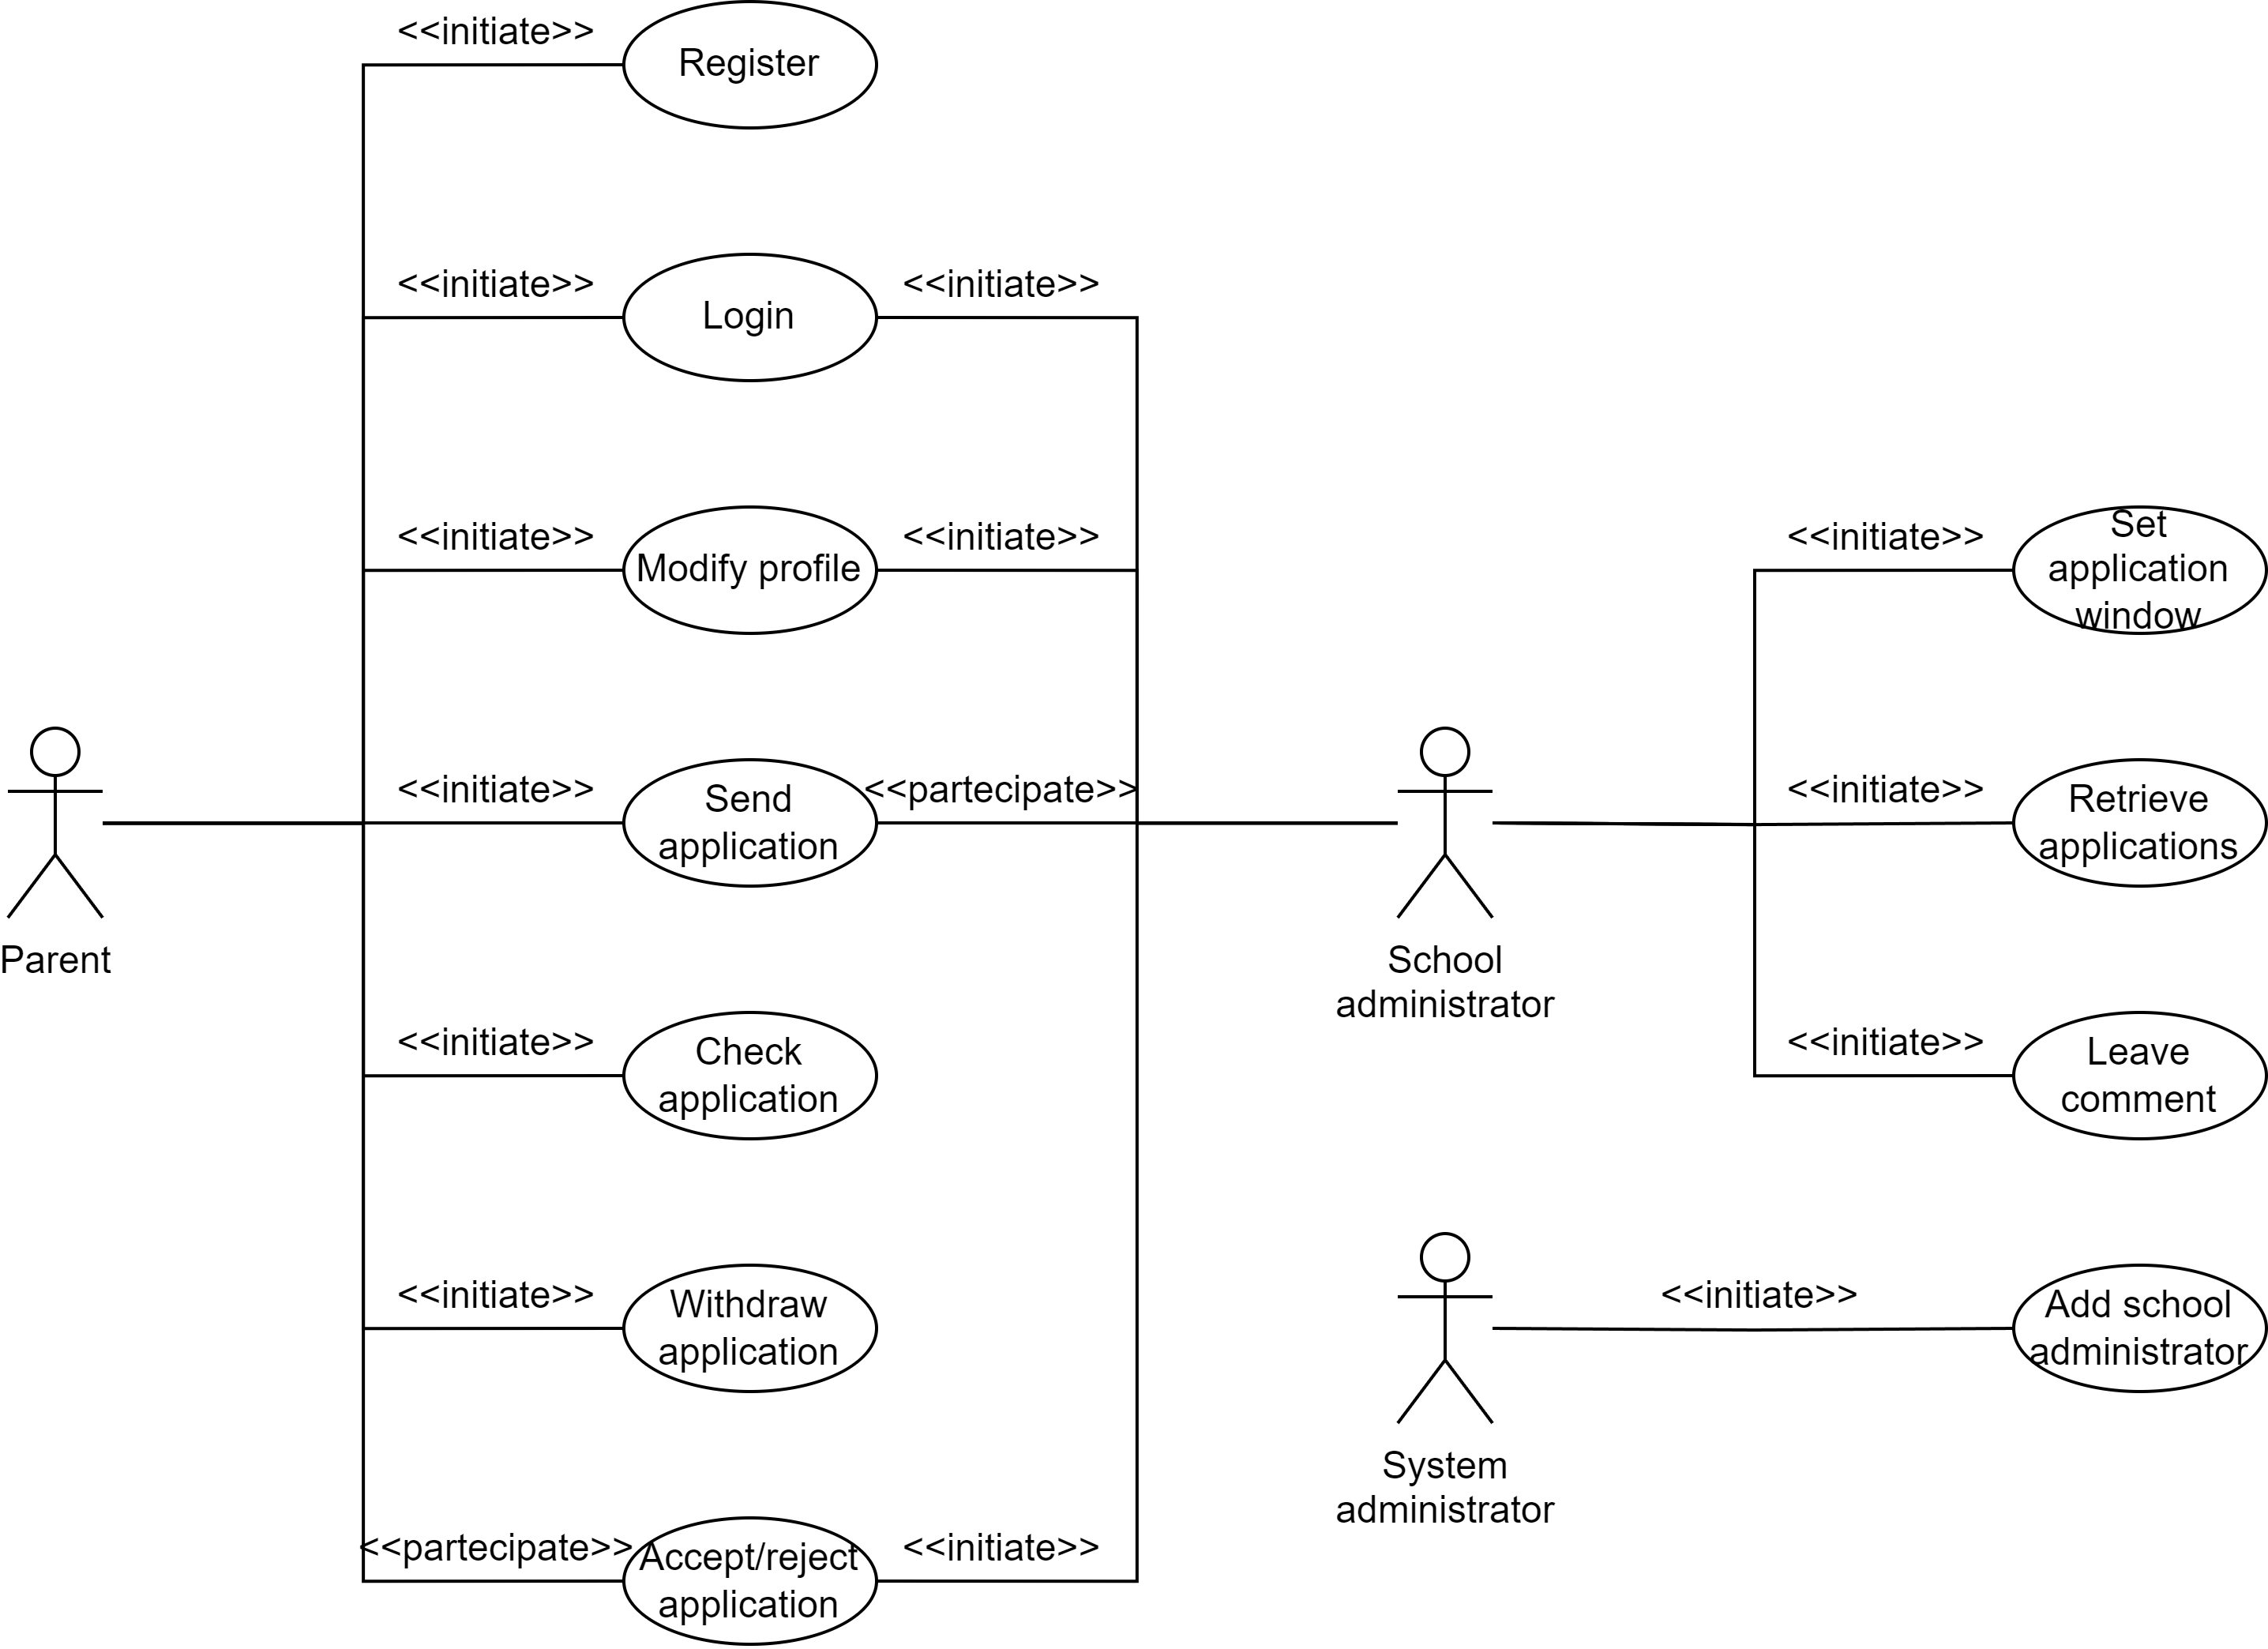
\includegraphics[width=1\linewidth]{images/usecase.png}
                \end{figure}
            \item We select send application case. We have that: 
                \begin{figure}[H]
                    \centering
                    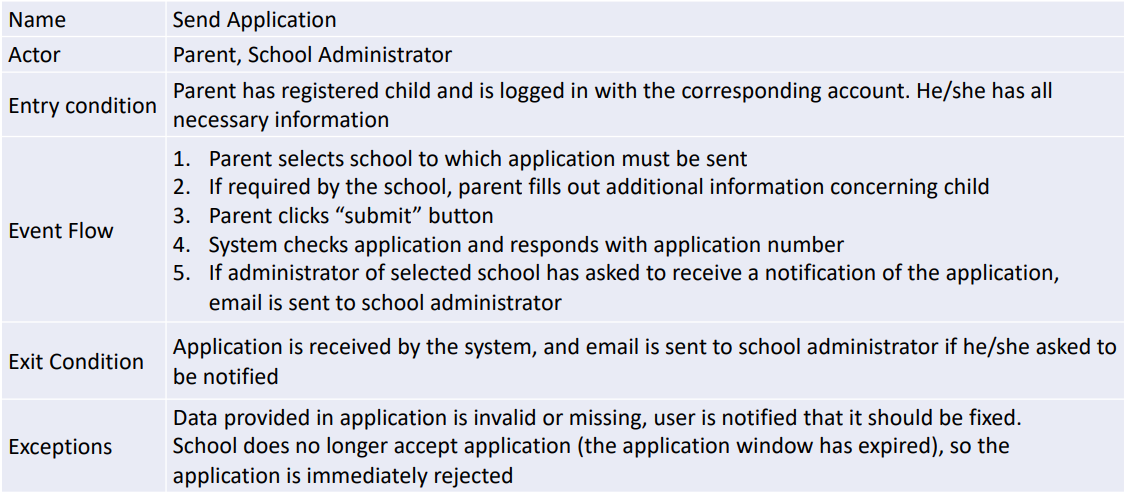
\includegraphics[width=0.9\linewidth]{images/sendapplication.png}
                \end{figure}
        \end{enumerate}
    \end{Answer}

    \newpage

    \begin{Exercise}[label=2]
        The private security and event organisation company HSG from the Netherlands wants to build an application (PaasPopCoin) that handles the coin emission and transactions in 
        the scope of a medium-size music festival they are organizing. The goal of the system is to allow festival-goers and operators to spend an allotted amount of money in 
        relative safety and without the need to bring wallets and other assets around the event. The software in question needs to handle at least three scenarios:
        \begin{itemize}
            \item Emission of coins in exchange for money through appropriate cashier desks and ATMs.
            \item Cash-back, that is, exchange of coins with cash in the same locations (we assume that people at the festival may be willing to receive back the money corresponding
                to the coins they have not used).
            \item Tracking of coin expenditure transactions at the various festival shops.
        \end{itemize}
        In the scope of the above scenarios, there are several special conditions to be considered. First, in the scope of coin emissions, there exist four classes of coin buyers: 
        \begin{itemize}
            \item [a.] VIPs who receive a $30\%$ discount on the coins they buy. 
            \item [b.] Event organization people who receive a $50\%$ discount. 
            \item [c.] Event ticket holders class A, who receive a $20\%$ discount. 
            \item [d.] Regular ticket holders who receive no discount.
        \end{itemize}
        When buying coins, users first need to authenticate themselves by inserting their own ID card in the ATM or by giving it to the cashier; this allows the system to determine 
        the class to which each coin buyer belongs. After authentication, buyers get the coins upon inserting into the ATM or giving to the cashier the corresponding amount of money.
        Second, also in the context of cash-back, users need to authenticate with their ID card to make sure the appropriate amount of money is given back, considering their role and 
        privileges. Third, during the event, every shop clerk keeps track through the PaasPopCoin system of the sales of products and the coins received. PaasPopCoin relies on a 
        third-party analytics service to periodically check whether the festival is earning money or not (cost-benefit analysis). Such check is performed with respect to costs of 
        products being sold during the event, as well as the overhead to cover all event organization and management expenses. 
        \begin{enumerate}
            \item With reference to the Jackson-Zave distinction between the world and the machine, identify the relevant world phenomena for PaasPopCoin, including the ones shared 
                with the machine, providing a short description if necessary. For shared phenomena specify whether they are controlled by the world or the machine. Focus on phenomena 
                that are relevant to describe the requirements of the system.
            \item Describe through a UML Class Diagram the main elements of the PaasPopCoin domain. 
            \item Define a UML Use Case Diagram describing the relevant actors and use cases for PaasPopCoin. You can provide a brief explanation of the Use Case Diagram, especially 
                if the names of the use cases are not self-explanatory.
        \end{enumerate}
    \end{Exercise}
    \begin{Answer}[ref=2]
        \begin{enumerate}
            \item The world-only phenomena can be: 
                \begin{itemize}
                    \item User buys Class A ticket.
                    \item User buys regular ticket.
                    \item VIP is contracted for event.
                    \item Event organization is started and contractors registered.
                    \item Event starts.
                    \item User gives money to cashier (to be converted in coins).
                    \item User gives coins to cashier (to be converted in money).
                    \item User gives ID card to cashier.
                    \item User buys some product at festival.
                    \item The external analytics service checks the success of an event.
                \end{itemize}

                The shared phenomena can be the following: 
                \begin{itemize}
                    \item User inserts money into an ATM machine.
                    \item ID Card is inserted into ATM.
                    \item User inserts coins into an ATM.
                    \item Cashier inserts in the system an ID card number.
                    \item Cashier inserts in the system the amount of money handed by a certain user.
                    \item Cashier inserts in the system the amount of coins returned by a certain user.
                    \item Store clerk inputs in system the amount of coins spent by user in shop.
                    \item The system enables coin emission after checking ID card and inserted amount of money.
                    \item The system enables cash-back after checking ID card and inserted number of coins.
                    \item The system sends data about purchases to the external analytics service.
                \end{itemize}
            \item The UML diagram of the given problem is: 
                \begin{figure}[H]
                    \centering
                    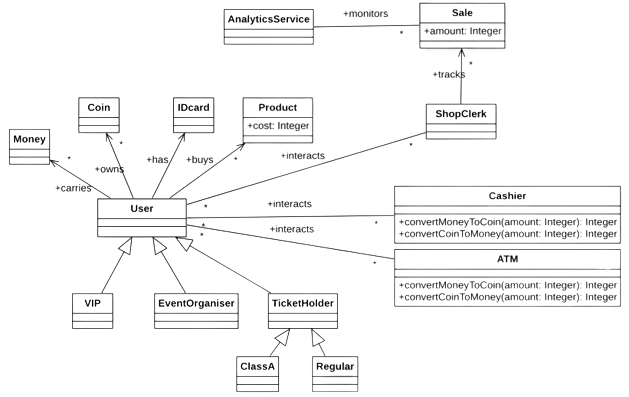
\includegraphics[width=0.9\linewidth]{images/UML.png}
                \end{figure}
            \item The UML use case diagram diagram of the given problem is: 
                \begin{figure}[H]
                    \centering
                    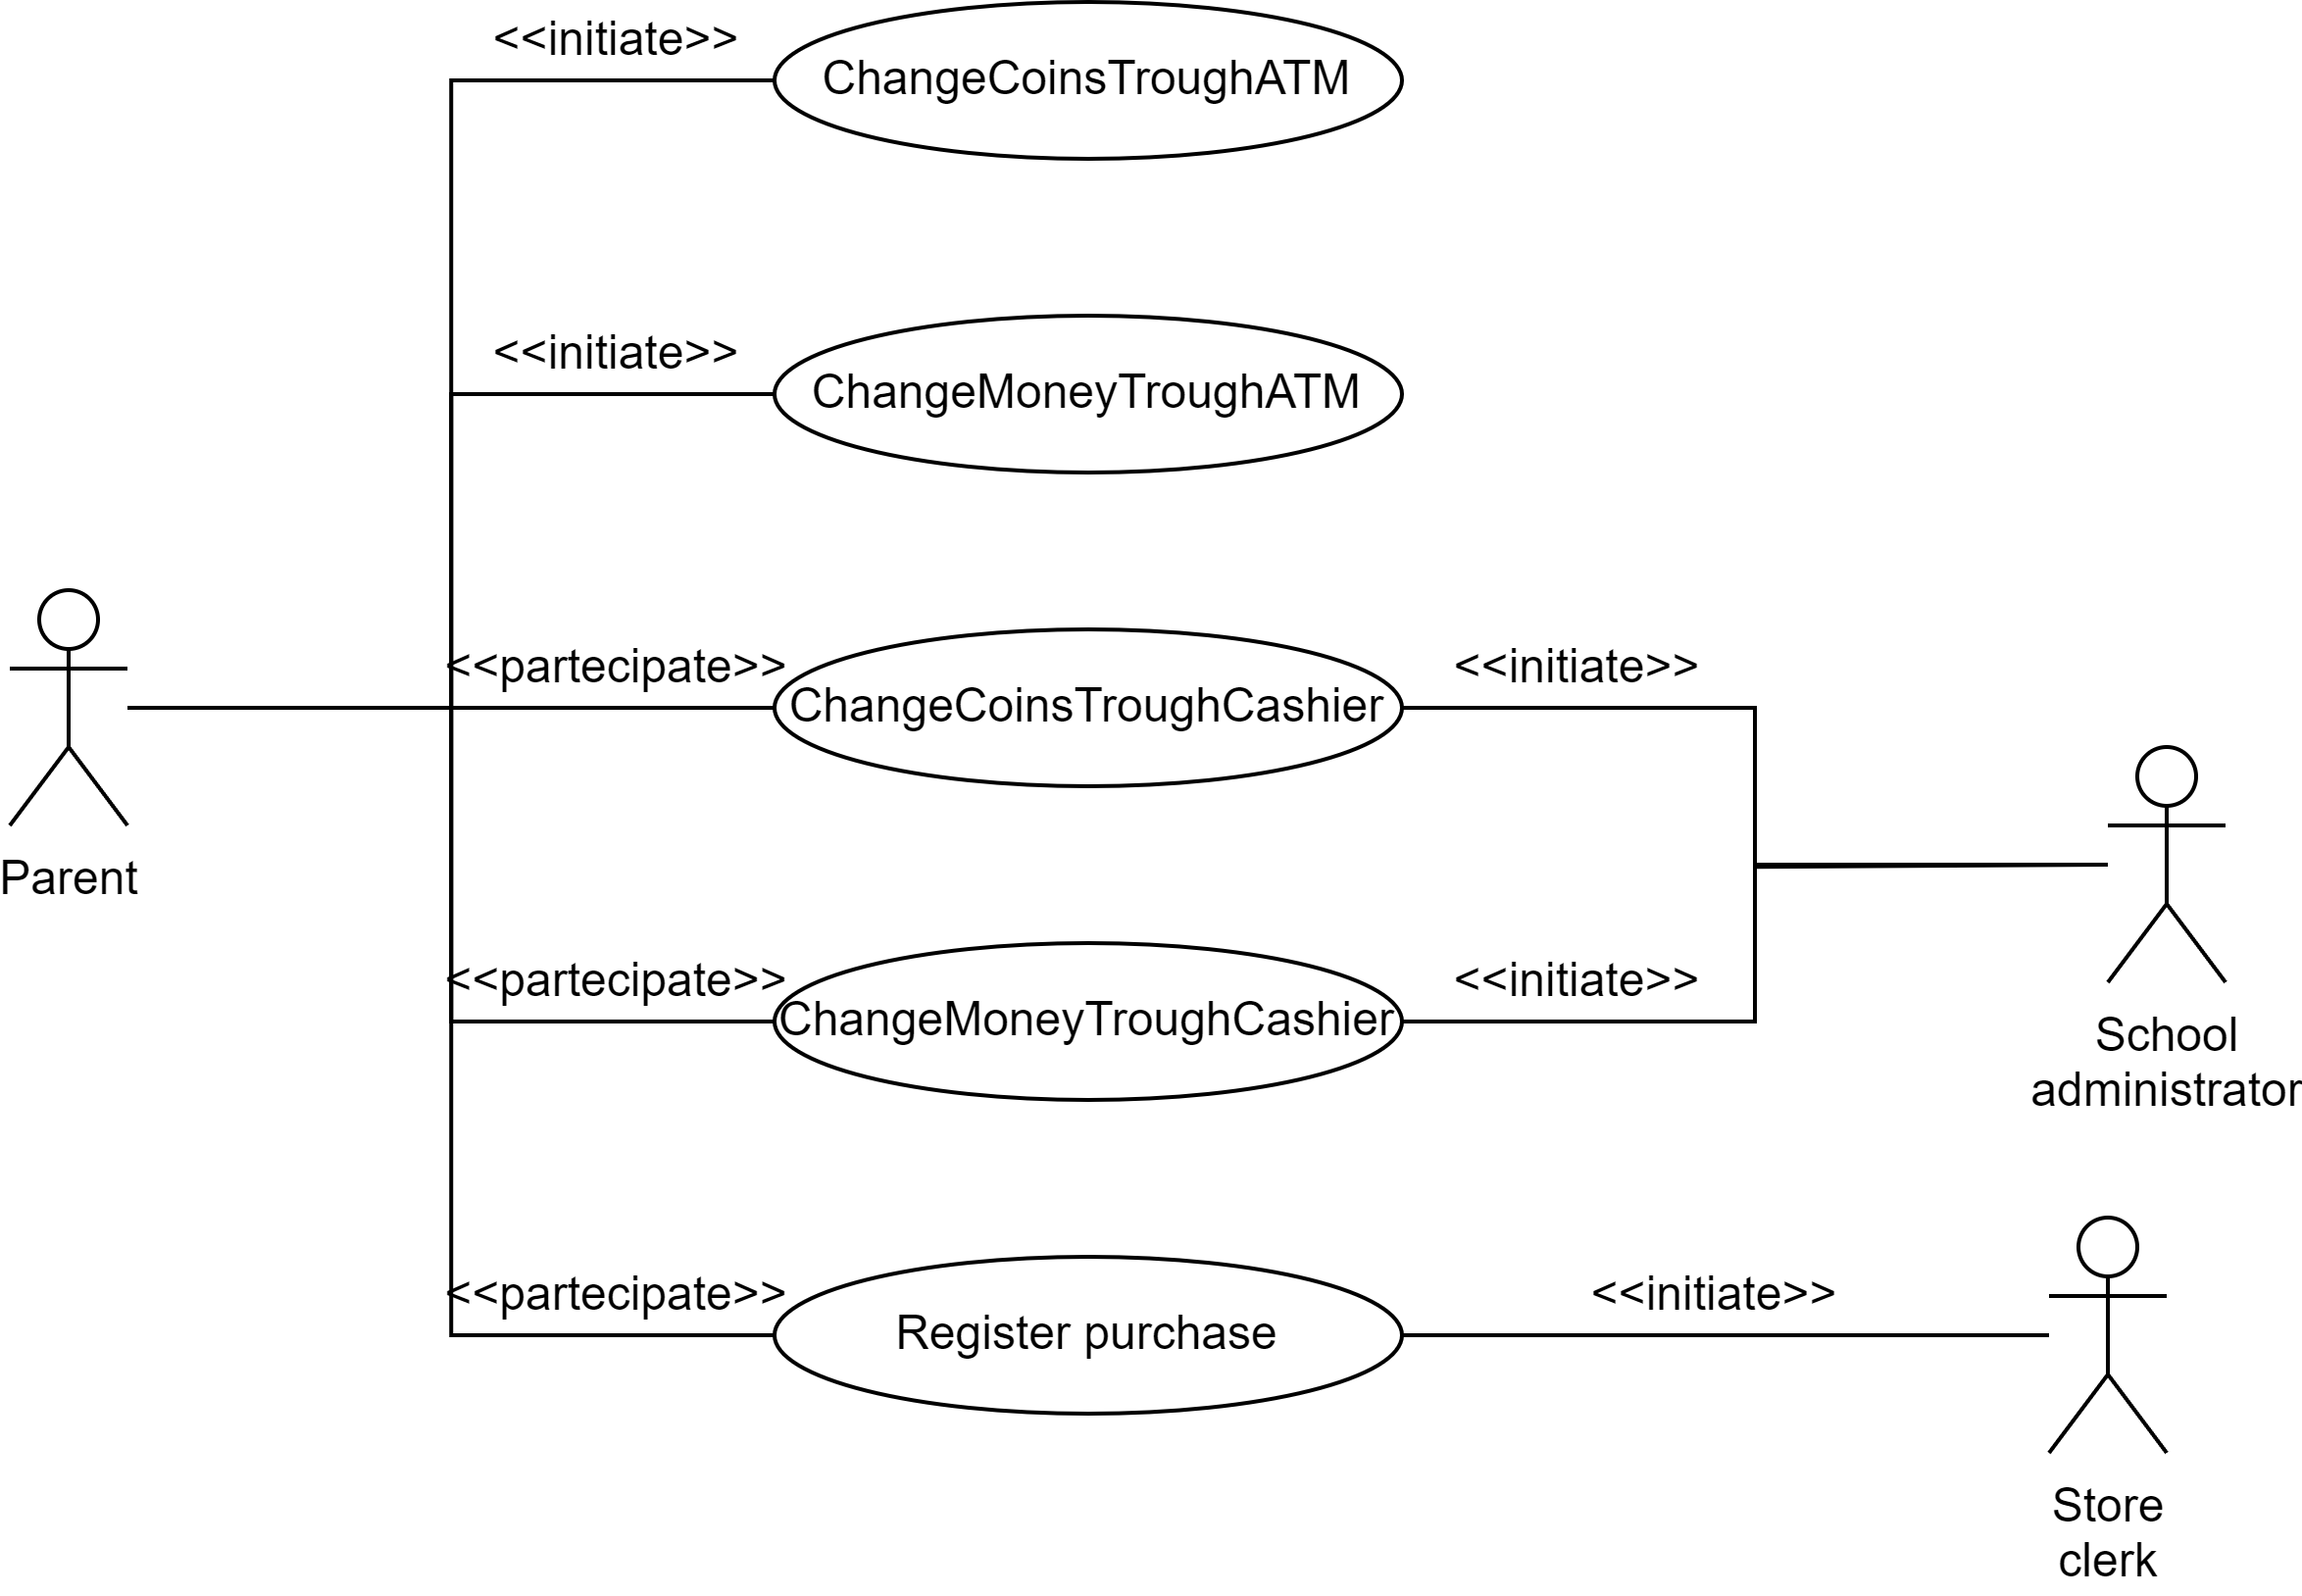
\includegraphics[width=0.9\linewidth]{images/usecase2.png}
                \end{figure}
        \end{enumerate}
    \end{Answer}
\end{document}